% PocketDRS one-page marketing explainer (general audience, plain English).
% Build: xelatex pocketdrs_onepager.tex   (needs the Poppins Google font)
\documentclass[11pt]{article}
\usepackage[a4paper,top=0.7cm,bottom=0.6cm,left=1.1cm,right=1.1cm]{geometry}
\usepackage{graphicx}
\usepackage[dvipsnames]{xcolor}
\usepackage{tikz}
\usetikzlibrary{calc}
\usepackage{fontspec}

% Poppins: a clean, friendly Google font. Regular body, SemiBold emphasis,
% Bold/Black display. No italic shipped, so map italic to Regular.
\setmainfont{Poppins}[
  Path = \detokenize{/Users/nirajkafle/Library/Fonts/} ,
  Extension = .ttf ,
  UprightFont = *-Regular , BoldFont = *-SemiBold ,
  ItalicFont = *-Regular , BoldItalicFont = *-SemiBold ]
\newfontfamily\displayfont{Poppins}[
  Path = \detokenize{/Users/nirajkafle/Library/Fonts/} ,
  Extension = .ttf , UprightFont = *-Bold ]
\newfontfamily\heavyfont{Poppins}[
  Path = \detokenize{/Users/nirajkafle/Library/Fonts/} ,
  Extension = .ttf , UprightFont = *-Black ]

\definecolor{navy}{RGB}{14,38,68}
\definecolor{ball}{RGB}{230,92,36}
\definecolor{grass}{RGB}{31,148,92}
\definecolor{ink}{RGB}{44,50,58}
\definecolor{paleblue}{RGB}{237,242,248}
\definecolor{line}{RGB}{208,216,226}

\setlength{\parindent}{0pt}
\setlength{\parskip}{0pt}
\linespread{1.1}
\pagestyle{empty}
\color{ink}
\raggedright

% Uppercase tracked micro-label.
\newcommand{\lbl}[2]{{\addfontfeatures{LetterSpace=9.0}\scriptsize\color{#2}\MakeUppercase{#1}}}

% Section heading: orange tab + tracked navy title.
\newcommand{\sect}[1]{%
  {\color{ball}\rule[1.5pt]{22pt}{4pt}}\;%
  {\displayfont\Large\color{navy}\addfontfeatures{LetterSpace=1.0}#1}\par\vspace{2pt}}

% Rounded-clipped framed image (fixed height).
\newcommand{\shot}[2][height=5.3cm]{%
  \begin{tikzpicture}
    \node[inner sep=0pt, rounded corners=9pt, clip] {\includegraphics[#1,keepaspectratio]{#2}};
  \end{tikzpicture}}

% Full-width rounded-clipped hero image.
\newcommand{\herowide}[1]{%
  \begin{tikzpicture}
    \node[inner sep=0pt, rounded corners=11pt, clip] {\includegraphics[width=\linewidth]{#1}};
  \end{tikzpicture}}

\begin{document}

% ---- Header band -------------------------------------------------------- %

\begin{tikzpicture}
  \node[fill=white, draw=line, line width=1pt, rounded corners=14pt,
        text width=\dimexpr\textwidth-36pt,
        inner xsep=17pt, inner ysep=10pt, align=center] (hd) {%
    {\heavyfont\Huge\color{navy}\addfontfeatures{LetterSpace=1.5}PocketDRS}\\[4pt]
    {\large\color{ink}Hawk-Eye LBW review from a single phone}\\[3pt]
    \lbl{Pocket Decision Review System}{grass}};
\end{tikzpicture}

\vspace{6pt}

% ---- Slim tagline strip (no accuracy / verdict claims up top) ----------- %

\begin{tikzpicture}
  \node[fill=paleblue, rounded corners=9pt, text width=\dimexpr\textwidth-22pt,
        align=center, inner ysep=7pt] {%
    \displayfont\normalsize
    {\color{grass}1}~\lbl{phone}{navy}\quad\textbullet\quad
    {\color{ink}Rs\,0}~\lbl{extra hardware}{navy}\quad\textbullet\quad
    {\color{ball}3-D}~\lbl{TV-style replay}{navy}};
\end{tikzpicture}

\vspace{7pt}

% ---- Both images in one row: 3-D review (wide) + on-video clip (tall) --- %
\noindent
\begin{minipage}[t]{0.73\textwidth}
  \shot[width=\linewidth]{../validation/test3/test3_3d_app.png}\\[3pt]
  {\footnotesize\color{navy}The delivery reviewed in 3-D, just like on TV.}
\end{minipage}\hfill
\begin{minipage}[t]{0.255\textwidth}
  \centering
  \shot[height=8.5cm]{../validation/test3/test3_sample.png}\\[3pt]
  {\footnotesize\color{navy}The same ball on your phone video.}
\end{minipage}

\vfill

% ---- What is it --------------------------------------------------------- %
\sect{What is it?}
In cricket, an umpire must judge whether a ball that hit the batter's leg would
have gone on to hit the stumps (an LBW). On TV this needs costly \textbf{Hawk-Eye}
cameras. \textbf{PocketDRS gives the same answer from just one phone}, as a clear,
TV-style replay.

\vfill

% ---- How it works: slim numbered step strip ----------------------------- %
\sect{How it works}
\vspace{3pt}
\newcommand{\stpbadge}[2]{{\tikz[baseline=-3pt]\node[fill=#2,circle,text=white,%
  minimum size=15pt,inner sep=0pt,font=\displayfont\scriptsize]{#1};}}

\begin{tikzpicture}
  \node[fill=paleblue, rounded corners=9pt, text width=\dimexpr\textwidth-22pt,
        align=center, inner ysep=8pt] {%
    \small
    \stpbadge{1}{grass}~\textbf{Mark} the pitch \& stumps\quad
    \stpbadge{2}{navy}~\textbf{Find} the ball\quad
    \stpbadge{3}{ball}~\textbf{Rebuild} in 3-D\quad
    \stpbadge{4}{ink}~\textbf{Decide} the verdict};
\end{tikzpicture}

\vfill

% ---- Proof + limit ------------------------------------------------------ %
\sect{Does it work?}
\vspace{2pt}
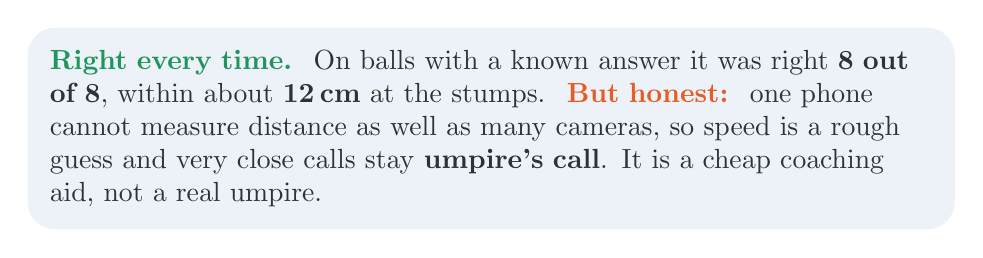
\begin{tikzpicture}
  \node[fill=paleblue, rounded corners=10pt,
        text width=\dimexpr\textwidth-26pt, inner sep=8pt] {%
    \color{ink}\setlength{\parindent}{0pt}\linespread{1.12}\selectfont
    {\bfseries\color{grass}Right every time.}\; On balls with a known answer it
    was right \textbf{8 out of 8}, within about \textbf{12\,cm} at the stumps.\;
    {\bfseries\color{ball}But honest:}\; one phone cannot measure distance as
    well as many cameras, so speed is a rough guess and very close calls stay
    \textbf{umpire's call}. It is a cheap coaching aid, not a real umpire.};
\end{tikzpicture}

\vfill

% ---- Footer bar --------------------------------------------------------- %

\begin{tikzpicture}
  \node[fill=paleblue, rounded corners=9pt, text width=\dimexpr\textwidth-28pt,
        inner ysep=9pt, inner xsep=14pt, align=center] {%
    \lbl{Niraj Kafle \textbullet\ Phoenix College of Management \textbullet\ Lincoln University}{navy}};
\end{tikzpicture}

\end{document}
